\subsection{Casos de test}

Evaluamos\footnote{El script asociada se puede encontrar en \textit{./experimentos/convergencia.py}, los archivos resultado en \textit{./experimentos/resultados/convergencia-iterativos}} el error absoluto en norma $L_1$ de los resultados de nuestra implementación de PageRank sobre el \textit{método de Jacobi} y el \textit{método de Gauss-Seidel} para los casos no triviales de test provistos por la cátedra\footnote{Los mismos se pueden encontrar en \textit{./catedra/tests-pagerank}}, en función de la cantidad de iteraciones realizadas.

\vspace{2em}
\noindent\textsc{Metodología}. Se evaluó el error absoluto $||x - $PageRank(g,\ p)$||_1$, donde $x$ refiere a la solución verdadera, $g$ refiere al grafo de entrada y $p$ al \textit{valor p}\footnote{Para una explicación en más detalle de PageRank, ver el $tp1$.}, para cada caso de test provisto, en función de la cantidad de iteraciones $q$ en el rango $[1, 100]$.

Se repitió el experimento para dos implementaciones del algoritmo que difieren únicamente en el método utilizado para la resolución del sistema lineal asociado al problema. En el primer caso se utilizó el \textit{método de Jacobi} y en el segundo el \textit{método de Gauss-Seidel}. Se controló la tolerancia ($t = 0$) para forzar a los algoritmos a iterar de manera exacta. 

\vspace{2em}
\noindent\textsc{Resultados}. Procedemos a mostrar de manera gráfica los resultados del error absoluto $L_1$ para cada caso de test:

\vspace{1em}
\begin{figure}[!htbp]
    %\ContinuedFloat
    \centering
    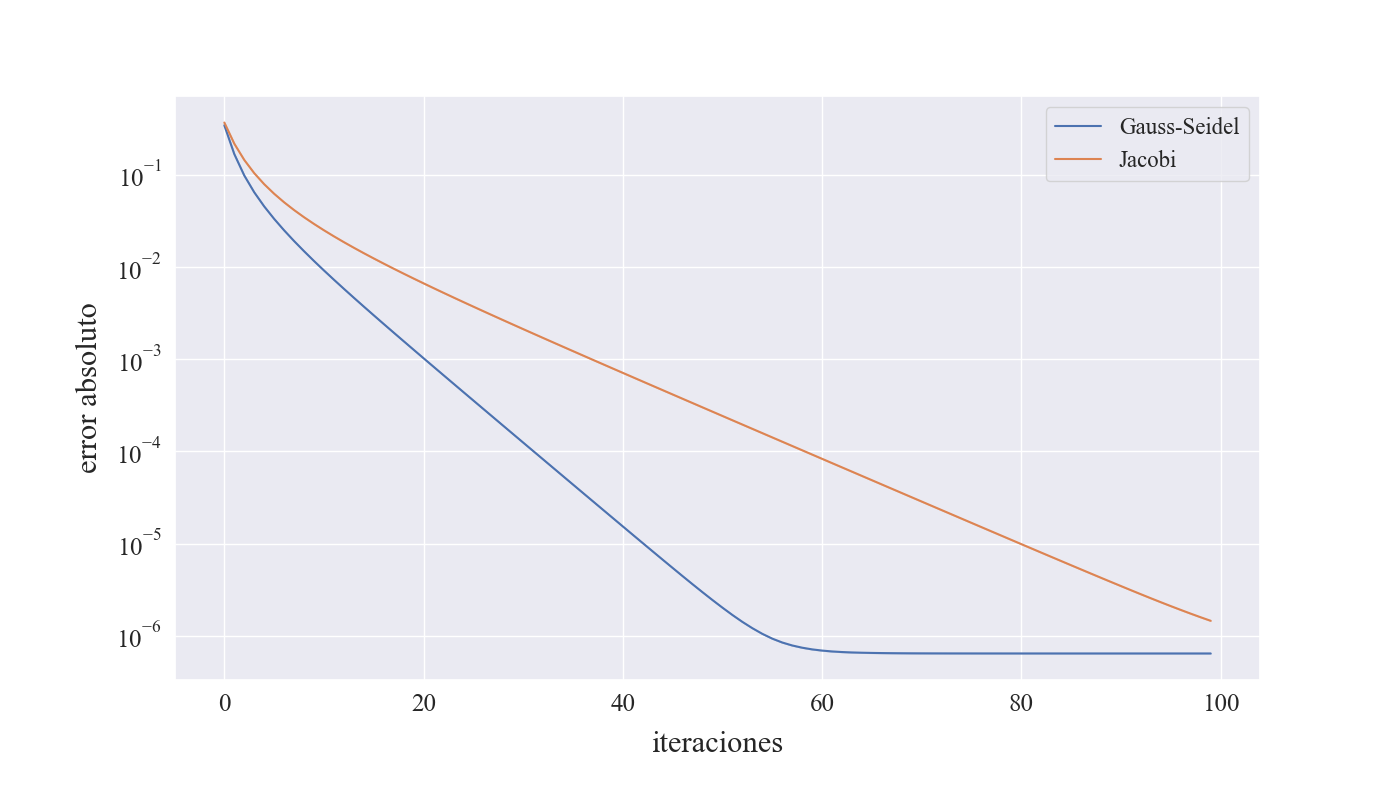
\includegraphics[width=1\textwidth]{files/src/.media/convergencia_test_15_segundos.png}
    \caption{Error absoluto $L_1$ para el grafo del test \textit{15\_segundos}, con $n = 2000$ y $p = 0.9$, en función de la cantidad de iteraciones realizadas, para los métodos de \textit{Jacobi} y \textit{Gauss-Seidel}.} \label{test_15_segundos}
\end{figure}

%\vspace{1em}
\newpage
\begin{figure}[!htbp]
    %\ContinuedFloat
    \centering
    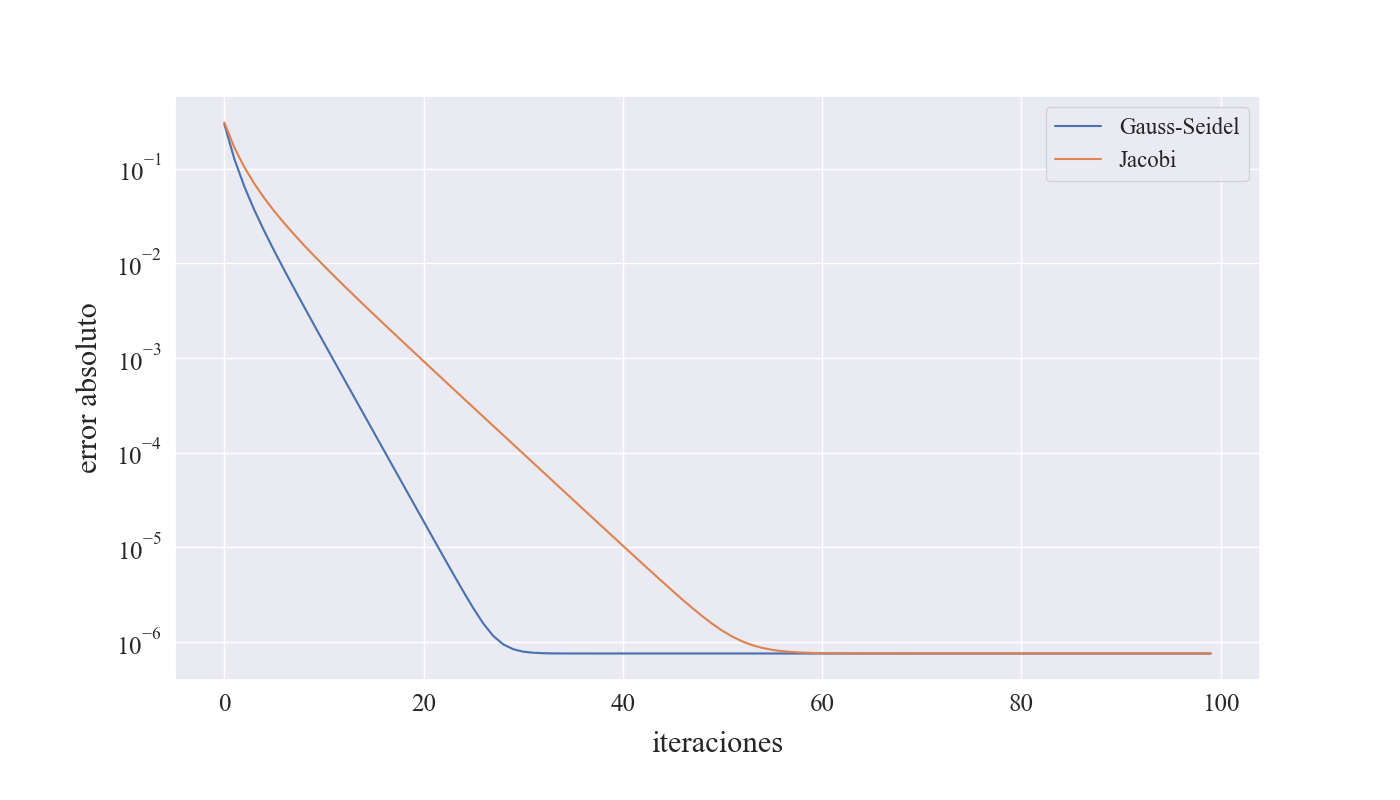
\includegraphics[width=1\textwidth, trim=0 0 0 30]{files/src/.media/convergencia_test_30_segundos.png}
    \caption{Error absoluto $L_1$ para el grafo del test \textit{30\_segundos}, con $n = 3000$ y $p = 0.8$, en función de la cantidad de iteraciones realizadas, para los métodos de \textit{Jacobi} y \textit{Gauss-Seidel}.} \label{test_30_segundos}
\end{figure}

%\vspace{1em}
\begin{figure}[!htbp]
    %\ContinuedFloat
    \centering
    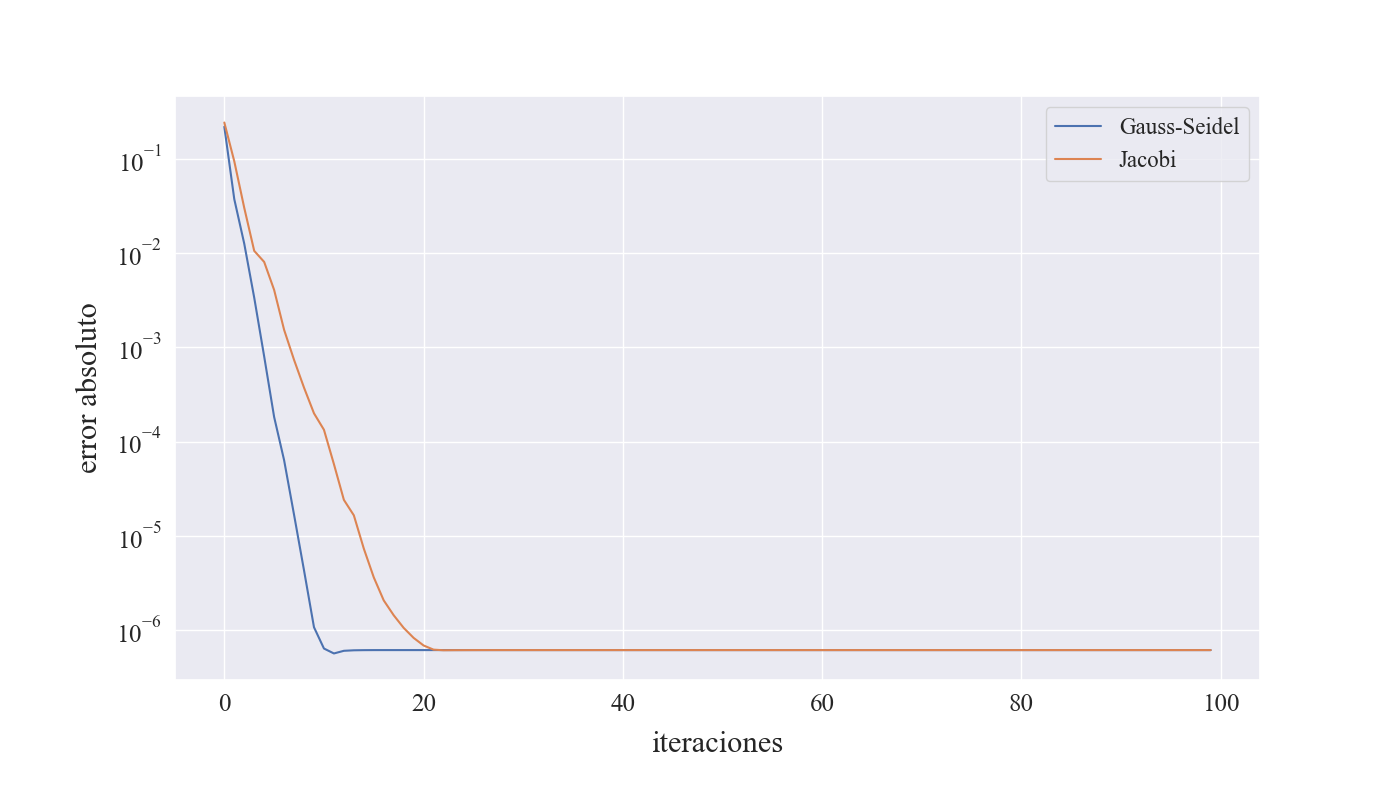
\includegraphics[width=1\textwidth, trim=0 0 0 30]{files/src/.media/convergencia_test_aleatorio_desordenado.png}
    \caption{Error absoluto $L_1$ para el grafo del test \textit{aleatorio\_desordenado}, con $n = 5$ y $p = 0.76$, en función de la cantidad de iteraciones realizadas, para los métodos de \textit{Jacobi} y \textit{Gauss-Seidel}.} \label{test_aleatorio_desordenado}
\end{figure}

%\vspace{1em}
\begin{figure}[!htbp]
    %\ContinuedFloat
    \centering
    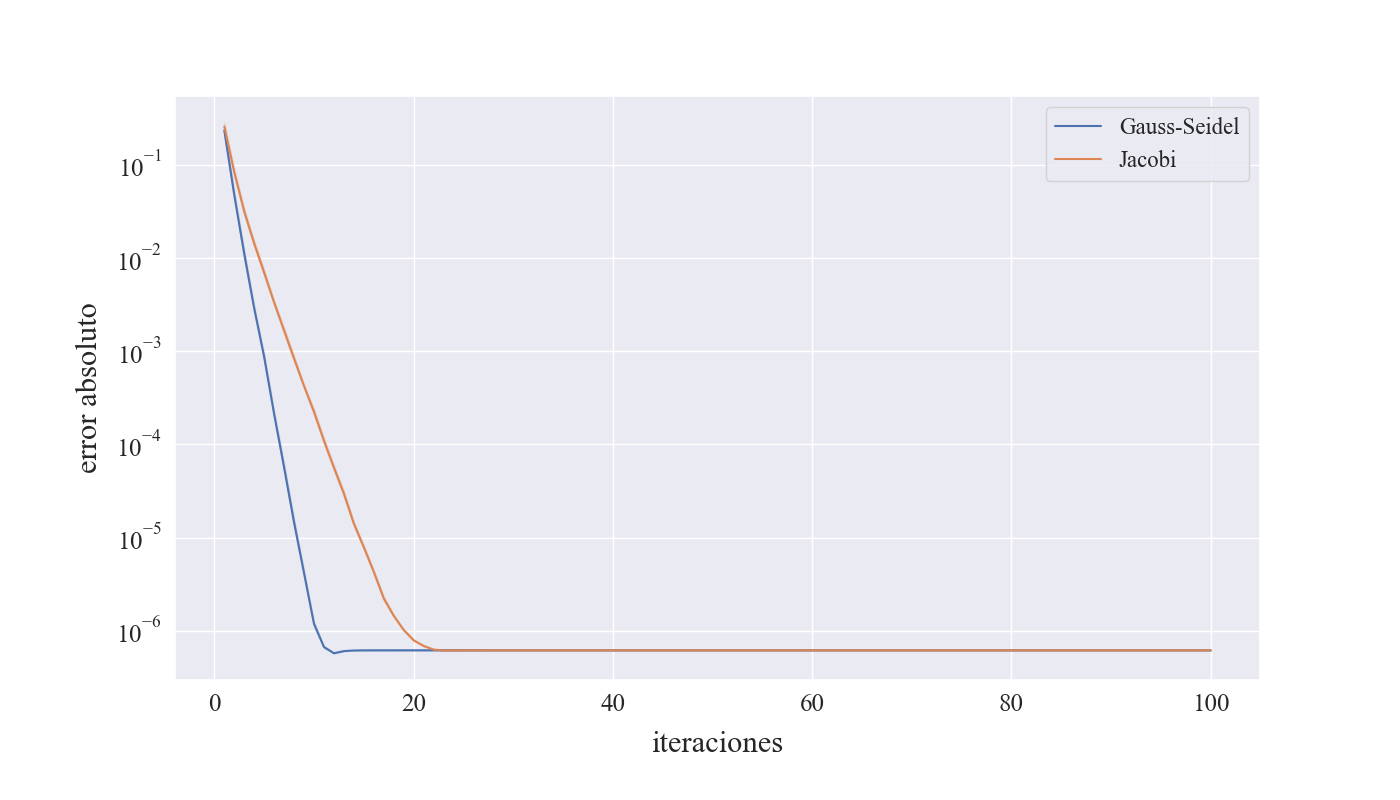
\includegraphics[width=1\textwidth]{files/src/.media/convergencia_test_aleatorio.png}
    \caption{Error absoluto $L_1$ para el grafo del test \textit{aleatorio}, con $n = 5$ y $p = 0.76$, en función de la cantidad de iteraciones realizadas, para los métodos de \textit{Jacobi} y \textit{Gauss-Seidel}.} \label{test_aleatorio}
\end{figure}

%\vspace{1em}
\begin{figure}[!htbp]
    %\ContinuedFloat
    \centering
    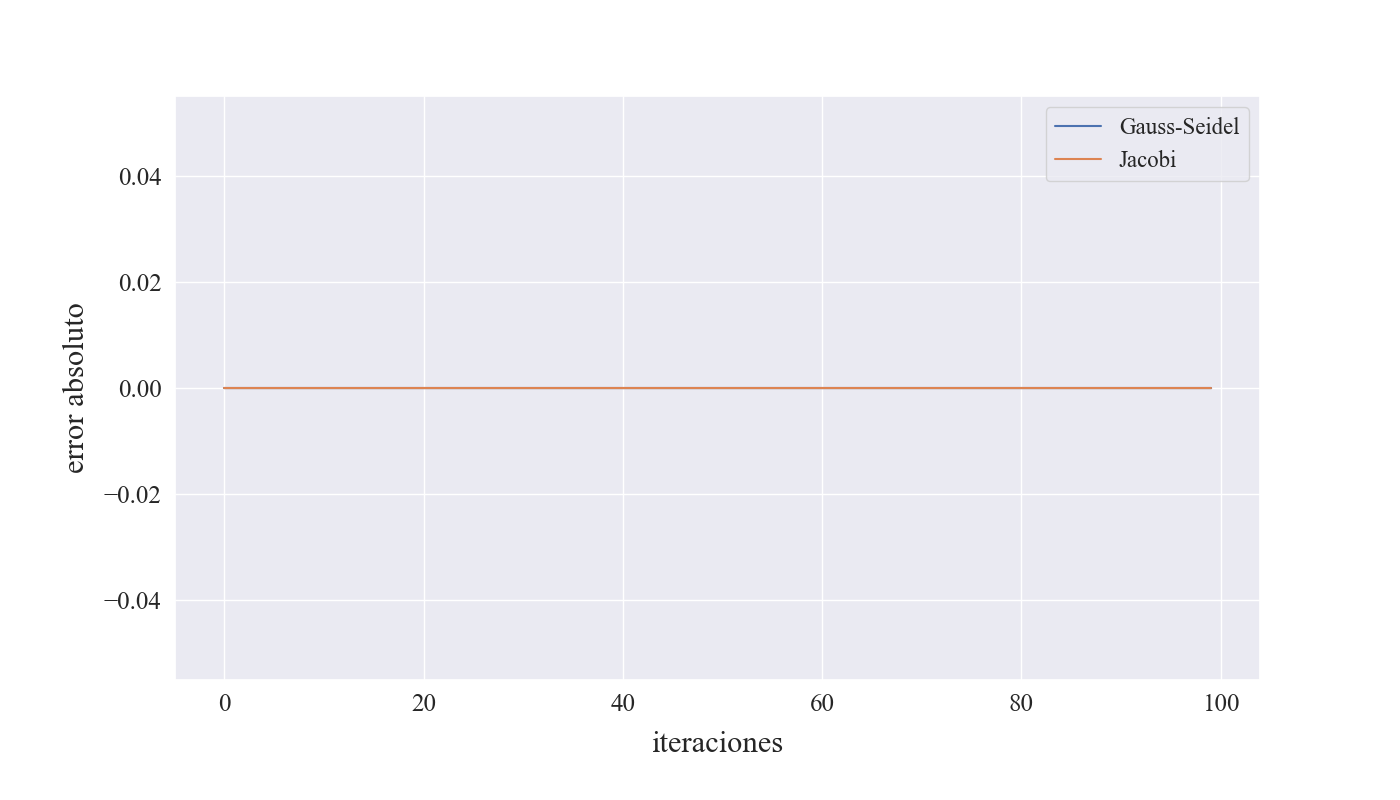
\includegraphics[width=1\textwidth]{files/src/.media/convergencia_test_sin_links.png}
    \caption{Error absoluto $L_1$ para el grafo del test \textit{sin\_links}, con $n = 5$ y $p = 0.64$, en función de la cantidad de iteraciones realizadas, para los métodos de \textit{Jacobi} y \textit{Gauss-Seidel}.} \label{test_sin_links}
\end{figure}
